\section{Experimental Evaluation}\label{sec:results}
We modified Falcon's~\cite{falcon} abstract syntax tree (AST) processing and code generation to generate various types of codes presented in the last section.
For CPUs, it generates OpenMP code, while for GPU and multi-GPU targets, it generates CUDA code.

\subsection{Experimental Setup}\label{expt:setup}
We used a range of graph types to assess the effectiveness of our proposal.
The dataset graphs in our experimental setup and their characteristics are presented in Table~\ref{expt:chars}.
We used four graph algorithms in our testbed: Breadth-First Search (BFS), Connected Components (CC), Minimum Spanning Tree computation (MST) and Single-Source Shortest Paths computation (SSSP).
All these algorithms are fundamental in graph theory and form building blocks in various application domain.
We compare the generated codes against the following frameworks: Galois~\cite{Pingali:2011:TPA:1993316.1993501}, Totem~\cite{Gharaibeh:2012:YOT:2370816.2370866}, Green-Marl~\cite{Hong:2012:GDE:2150976.2151013}, LonestarGPU~\cite{nasre13:MAG:2517327.2442531} and Gunrock~\cite{Wang:2016:GHG:3016078.2851145}.
In the sequel, Falcon refers to our proposed techniques embedded into existing Falcon.

The CPU benchmarks for OpenMP are run on an Intel XeonE5-2650 v2 machine with 32 cores clocked at 2.6 GHz with 100 GB RAM, 32KB of L1 data cache, 256KB of L2 cache and 20MB of L3 cache. The machine runs CentOS 6.5 and 2.6.32-431 kernel, with GCC version 4.4.7 and OpenMP version 4.0. The CUDA code is run on Tesla K40C devices each having 2880 cores clocked at 745 MHz with 12GB of global memory. Eight similar GPU devices are connected to the same CPU device.

\begin{figure}
\begin{minipage}{0.45\textwidth}
\begin{table}[H]
\centering
\footnotesize
\begin{tabular}{|l|r|r|r|}
\hline
Graph	& \#nodes	& \#edges	& max-degree	\\
	& $\times10^6$	& $\times10^6$	& \\
\hline
USA-road-CTR	& 14	& 34 	& 9    \\
USA-road-USA	& 24	& 58 	& 9    \\
soc-orkut-dir	& 3	& 234 	& 33313 \\
soc-sinaweibo	& 21	& 261 	& 278491 \\
random-25M	& 25	& 100 	& 17   \\
random-50M	& 50	& 200 	& 18   \\
random-75M	& 75	& 300 	& 18   \\
random-100M	& 100	& 400 	& 18   \\
random-125M	& 125	& 500 	& 19   \\
rmat-10M	& 10	& 100 	& 1873 \\
rmat-20M	& 20	& 200 	& 2525 \\
rmat-30M	& 30	& 300 	& 3796 \\
rmat-40M	& 40	& 400 	& 3333 \\
rmat-50M	& 50	& 500 	& 4132 \\
\hline
\end{tabular}
\caption{Benchmark characteristics}
\label{expt:chars}
\end{table}
\end{minipage}\hfill
\begin{minipage}{0.45\textwidth}
\begin{table}[H]
\centering
\footnotesize
\begin{tabular}{|l|r|r|r|r|}
\hline
Graph	 	& BFS	& CC	& MST	& SSSP \\
\hline
USA-road-CTR	& 3456	& 14103	& 727	& 30299 \\
USA-road-USA	& 9113	& 24061	& 779	& 72857 \\
soc-orkut-dir	& 269	& 623	& 5509	& 267   \\
soc-sinaweibo	& 1234	& 1955	& 30556	& 1151  \\
random-25M	& 131	& 411	& 2832	& 561   \\
random-50M	& 270	& 823	& 6665	& 1142  \\
random-75M	& 414	& 1416	& 11265	& 1796  \\
random-100M	& 583	& 2192	& 15860	& 2413  \\
random-125M	& 756	& 2909	& 25973	& 3194  \\
rmat-10M	& 133	& 387	& 2770	& 536   \\
rmat-20M	& 266	& 789	& 6240	& 1169  \\
rmat-30M	& 424	& 893	& 8963	& 1859  \\
rmat-40M	& 542	& 1601	& 13232	& 2405  \\
rmat-50M	& 707	& 2026	& 16825	& 3808  \\
\hline                                   
\textbf{Total}		& 18298	& 54189	& 148196&  123457 \\
\hline
\end{tabular}
\caption{Baseline times (ms) of Falcon on GPU}
\label{expt:baselines}
\end{table}
\end{minipage}
\end{figure}

\REM{
\begin{figure}
\centering
\includegraphics[width=0.99\linewidth]{SSSP.png}
\includegraphics[width=0.99\linewidth]{BFS.png}
\caption{Falcon versus other frameworks for SSSP and BFS. Baseline is Totem at 1.0.}
\label{expt:frameworks}
\end{figure}
}

\subsection{Baselines and Comparison with Other Frameworks}\label{expt:comparison}
The baseline execution times of Falcon on GPU are listed in Table~\ref{expt:baselines}.
We observe that the execution times on road networks are particularly high for propagation based algorithms such as BFS, SSSP and CC.
This occurs because unlike other graphs, road networks have large diameters, leading to many iterations of the algorithm.


\begin{figure*}
  \begin{subfigure}{0.6\textwidth}
   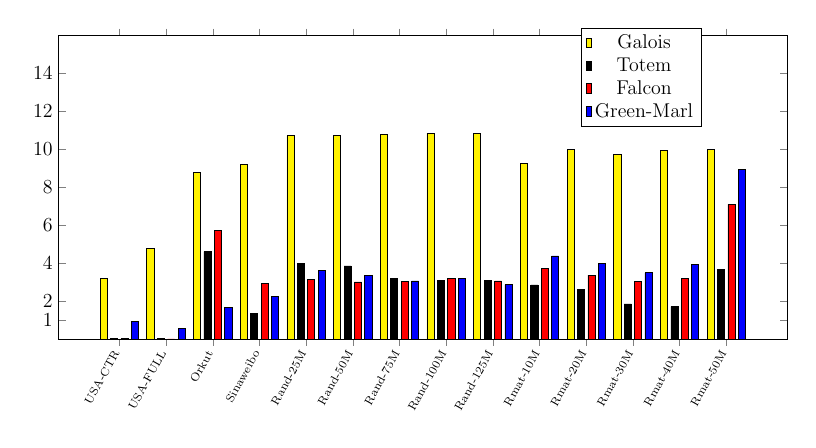
\begin{tikzpicture}[scale=0.6]
    \begin{axis}[
         ybar,% axis on top,
        ymin=0, ymax=16,
        height=8.0cm,
        width=17cm,
ytick={ 1,2,4,6,8,10,12,14},
%ymode=log,
 %       log basis y={2},
x tick label style={
rotate=60,anchor=east,font=\scriptsize},
        symbolic x coords={
           USA-CTR, USA-FULL, Orkut,Sinaweibo, Rand-25M,Rand-50M,Rand-75M,Rand-100M,Rand-125M, Rmat-10M,Rmat-20M,Rmat-30M,Rmat-40M,Rmat-50M
            },
       xtick=data,
        bar width=0.15cm,
%        major grid style={draw=black},
 %       enlarge y limits={value=.05,upper},
        % y tick style={grid=none},
         xticklabel style={rotate=1},
        %tickwidth=1pt,
       % enlarge x limits=true,
       legend style={
            at={(0.8,0.7)},
            anchor=south,
            legend columns=1,
           /tikz/every even column/.append style={font=\large}
        },
        legend entries={Lonestar-GPU,Falcon,Gunrock},
        legend image code/.code={%
      \draw[#1] (0cm,-0.1cm) rectangle (0.1cm,0.1cm);
   },  
        %ylabel={Speedup},
    %      nodes near coords,
  %nodes near coords align={vertical},
 every node near coord/.append style={color=black, rotate=90, anchor=south, font=\large},
             every axis/.append style={font=\large},
    ]
    \addplot [ fill=yellow] coordinates {
      (USA-CTR,3.18)
      (USA-FULL,4.76) 
      (Orkut, 8.77)
      (Sinaweibo,9.22)
      (Rand-25M,10.73)
      (Rand-50M,10.72) 
      (Rand-75M,10.81) 
      (Rand-100M,10.86) 
      (Rand-125M,10.86) 
      (Rmat-10M,9.28)
      (Rmat-20M,10.01) 
      (Rmat-30M,9.72) 
      (Rmat-40M,9.95) 
      (Rmat-50M,10.01) 
            };
    \addplot [ fill=black] coordinates {
      (USA-CTR,0.04)
      (USA-FULL,0.03) 
      (Orkut, 4.60)
      (Sinaweibo,1.33)
      (Rand-25M,3.97)
      (Rand-50M,3.85) 
      (Rand-75M,3.19) 
      (Rand-100M,3.08) 
      (Rand-125M,3.08) 
      (Rmat-10M,2.85)
      (Rmat-20M,2.62) 
      (Rmat-30M,1.85) 
      (Rmat-40M,1.7) 
      (Rmat-50M,3.65) 
            };
    \addplot [ fill=red] coordinates {
      (USA-CTR,0.01)
      (USA-FULL,0.00001) 
      (Orkut, 5.73)
      (Sinaweibo,2.94)
      (Rand-25M,3.16)
      (Rand-50M,3.01) 
      (Rand-75M,3.04) 
      (Rand-100M,3.2) 
      (Rand-125M,3.06) 
      (Rmat-10M,3.7)
      (Rmat-20M,3.36) 
      (Rmat-30M,3.02) 
      (Rmat-40M,3.21) 
      (Rmat-50M,7.1) 
            };
    \addplot [ fill=blue] coordinates {
      (USA-CTR,0.94)
      (USA-FULL,0.56) 
      (Orkut, 1.67)
      (Sinaweibo,2.25)
      (Rand-25M,3.61)
      (Rand-50M,3.34) 
      (Rand-75M,3.06) 
      (Rand-100M,3.2) 
      (Rand-125M,2.86) 
      (Rmat-10M,4.38)
      (Rmat-20M,3.99) 
      (Rmat-30M,3.49) 
      (Rmat-40M,3.95) 
      (Rmat-50M,8.93) 
            };
 \legend{\large{Galois},\large{Totem}, \large{Falcon},\large{Green-Marl}}
 \end{axis}
   \end{tikzpicture}
\caption{CPU: Speedup over Galois single thread}
\label{expt:ssspcpucompare}
\end{subfigure}%
  \begin{subfigure}{0.4\textwidth}
   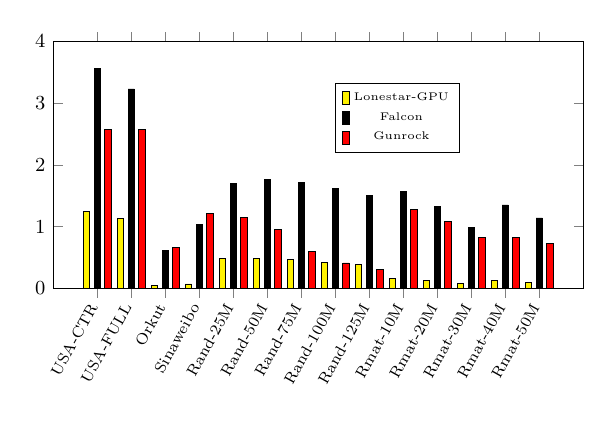
\begin{tikzpicture}[scale=0.8]
    \begin{axis}[
         ybar,% axis on top,
        ymin=0, ymax=4,
        height=5.5cm,
        width=10cm,
%ytick={0.5, 1,2,4,12,16},
x tick label style={
rotate=60,anchor=east,font=\scriptsize},
        symbolic x coords={
           USA-CTR, USA-FULL, Orkut,Sinaweibo, Rand-25M,Rand-50M,Rand-75M,Rand-100M,Rand-125M, Rmat-10M,Rmat-20M,Rmat-30M,Rmat-40M,Rmat-50M
            },
       xtick=data,
        bar width=0.1cm,
%        major grid style={draw=black},
 %       enlarge y limits={value=.05,upper},
        % y tick style={grid=none},
         xticklabel style={rotate=1},
        %tickwidth=1pt,
       % enlarge x limits=true,
       legend style={
            at={(0.65,0.55)},
            anchor=south,
            legend columns=1,
           /tikz/every even column/.append style={font=\tiny}
        },
        legend entries={Lonestar-GPU,Falcon,Gunrock},
        legend image code/.code={%
      \draw[#1] (0cm,-0.1cm) rectangle (0.1cm,0.1cm);
   },  
        %ylabel={Speedup},
    %      nodes near coords,
  %nodes near coords align={vertical},
 every node near coord/.append style={color=black, rotate=90, anchor=south, font=\tiny},
             every axis/.append style={font=\small},
    ]
    \addplot [ fill=yellow] coordinates {
      (USA-CTR,1.25)
      (USA-FULL,1.13) 
      (Orkut, 0.05)
      (Sinaweibo,0.07)
      (Rand-25M,0.49)
      (Rand-50M,0.49) 
      (Rand-75M,0.47) 
      (Rand-100M,0.42) 
      (Rand-125M,0.38) 
      (Rmat-10M,0.16)
      (Rmat-20M,0.13) 
      (Rmat-30M,0.08) 
      (Rmat-40M,0.13) 
      (Rmat-50M,0.10) 
            };
    \addplot [ fill=black] coordinates {
      (USA-CTR,3.56)
      (USA-FULL,3.23) 
      (Orkut, 0.62)
      (Sinaweibo,1.04)
      (Rand-25M,1.7)
      (Rand-50M,1.77) 
      (Rand-75M,1.72) 
      (Rand-100M,1.62) 
      (Rand-125M,1.51) 
      (Rmat-10M,1.57)
      (Rmat-20M,1.33) 
      (Rmat-30M,0.99) 
      (Rmat-40M,1.35) 
      (Rmat-50M,1.14) 
            };
    \addplot [ fill=red] coordinates {
      (USA-CTR,2.58)
      (USA-FULL,2.57) 
      (Orkut, 0.66)
      (Sinaweibo,1.22)
      (Rand-25M,1.15)
      (Rand-50M,0.96) 
      (Rand-75M,0.59) 
      (Rand-100M,0.41) 
      (Rand-125M,0.31) 
      (Rmat-10M,1.27)
      (Rmat-20M,1.08) 
      (Rmat-30M,0.83) 
      (Rmat-40M,0.82) 
      (Rmat-50M,0.73) 
            };
 \legend{Lonestar-GPU,Falcon, Gunrock}
 \end{axis}
   \end{tikzpicture}
\caption{GPU: Speedup over Totem}
\label{expt:ssspgpucompare}
\end{subfigure}%
\caption{SSSP comparison}
\label{expt:ssspcpugpu}
\end{figure*}


\begin{figure*}
\centering
  \begin{subfigure}{0.6\textwidth}
\centering
   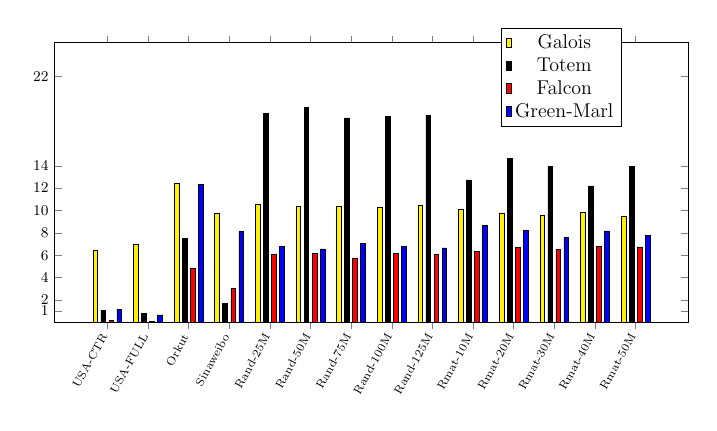
\begin{tikzpicture}[scale=0.6]
    \begin{axis}[
         ybar,% axis on top,
        ymin=0, ymax=25,
        height=7.5cm,
        width=15cm,
ytick={ 1,2,4,6,8,10,12,14,22},
%ymode=log,
 %       log basis y={2},
x tick label style={
rotate=60,anchor=east,font=\scriptsize},
        symbolic x coords={
           USA-CTR, USA-FULL, Orkut,Sinaweibo, Rand-25M,Rand-50M,Rand-75M,Rand-100M,Rand-125M, Rmat-10M,Rmat-20M,Rmat-30M,Rmat-40M,Rmat-50M
            },
       xtick=data,
        bar width=0.1cm,
%        major grid style={draw=black},
 %       enlarge y limits={value=.05,upper},
        % y tick style={grid=none},
         xticklabel style={rotate=1},
        %tickwidth=1pt,
       % enlarge x limits=true,
       legend style={
            at={(0.8,0.7)},
            anchor=south,
            legend columns=1,
           /tikz/every even column/.append style={font=\tiny}
        },
        legend entries={Lonestar-GPU,Falcon,Gunrock},
        legend image code/.code={%
      \draw[#1] (0cm,-0.1cm) rectangle (0.1cm,0.1cm);
   },  
      %  ylabel={Speedup},
    %      nodes near coords,
  %nodes near coords align={vertical},
 every node near coord/.append style={color=black, rotate=90, anchor=south, font=\tiny},
             every axis/.append style={font=\small},
    ]
    \addplot [ fill=yellow] coordinates {
      (USA-CTR,6.43)
      (USA-FULL,6.97) 
      (Orkut, 12.46)
      (Sinaweibo,9.78)
      (Rand-25M,10.51)
      (Rand-50M,10.35) 
      (Rand-75M,10.35) 
      (Rand-100M,10.32) 
      (Rand-125M,10.45) 
      (Rmat-10M,10.12)
      (Rmat-20M,9.75) 
      (Rmat-30M,9.54) 
      (Rmat-40M,9.81) 
      (Rmat-50M,9.49) 
            };
    \addplot [ fill=black] coordinates {
      (USA-CTR,1.09)
      (USA-FULL,0.82) 
      (Orkut, 7.54)
      (Sinaweibo,1.69)
      (Rand-25M,18.65)
      (Rand-50M,19.25) 
      (Rand-75M,18.28) 
      (Rand-100M,18.41) 
      (Rand-125M,18.5) 
      (Rmat-10M,12.73)
      (Rmat-20M,14.68) 
      (Rmat-30M,13.96) 
      (Rmat-40M,12.2) 
      (Rmat-50M,13.95) 
            };
    \addplot [ fill=red] coordinates {
      (USA-CTR,0.17)
      (USA-FULL,0.12) 
      (Orkut, 4.86)
      (Sinaweibo,3.01)
      (Rand-25M,6.04)
      (Rand-50M,6.16) 
      (Rand-75M,5.71) 
      (Rand-100M,6.2) 
      (Rand-125M,6.11) 
      (Rmat-10M,6.37)
      (Rmat-20M,6.73) 
      (Rmat-30M,6.54) 
      (Rmat-40M,6.77) 
      (Rmat-50M,6.75) 
            };
    \addplot [ fill=blue] coordinates {
      (USA-CTR,1.15)
      (USA-FULL,0.66) 
      (Orkut, 12.35)
      (Sinaweibo,8.1)
      (Rand-25M,6.81)
      (Rand-50M,6.57) 
      (Rand-75M,7.06) 
      (Rand-100M,6.79) 
      (Rand-125M,6.66) 
      (Rmat-10M,8.69)
      (Rmat-20M,8.24) 
      (Rmat-30M,7.57) 
      (Rmat-40M,8.17) 
      (Rmat-50M,7.76) 
            };
 %\legend{Galois,Totem, Falcon,Green-Marl}
 \legend{\large{Galois},\large{Totem}, \large{Falcon},\large{Green-Marl}}
 \end{axis}
   \end{tikzpicture}
\caption{CPU: Speedup Over Galois single thread}
\label{expt:bfscpucompare1}
\end{subfigure}%
  \begin{subfigure}{0.4\textwidth}
\centering
   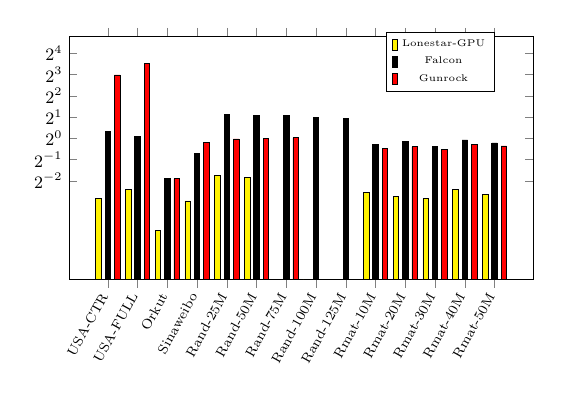
\begin{tikzpicture}[scale=0.7]
    \begin{axis}[
         ybar,% axis on top,
        ymin=0.01, ymax=28,
        height=6.0cm,
        width=10cm,
ymode=log,
log origin=infty,
        log basis y={2},
x tick label style={
rotate=60,anchor=east,font=\scriptsize},
        symbolic x coords={
           USA-CTR, USA-FULL, Orkut,Sinaweibo, Rand-25M,Rand-50M,Rand-75M,Rand-100M,Rand-125M, Rmat-10M,Rmat-20M,Rmat-30M,Rmat-40M,Rmat-50M
            },
       xtick=data,
ytick={0,0.25, 0.5, 1, 2,4,8,16},
        bar width=0.1cm,
%        major grid style={draw=black},
 %       enlarge y limits={value=.05,upper},
        % y tick style={grid=none},
         xticklabel style={rotate=1},
        %tickwidth=1pt,
       % enlarge x limits=true,
       legend style={
            at={(0.8,0.77)},
            anchor=south,
            legend columns=1,
           /tikz/every even column/.append style={font=\tiny}
        },
        legend entries={Lonestar-GPU,Falcon,Gunrock},
        legend image code/.code={%
      \draw[#1] (0cm,-0.1cm) rectangle (0.1cm,0.1cm);
   },  
        %ylabel={Speedup},
    %      nodes near coords,
  %nodes near coords align={vertical},
 every node near coord/.append style={color=black, rotate=90, anchor=south, font=\tiny},
             every axis/.append style={font=\small},
    ]
    \addplot [ fill=yellow] coordinates {
      (USA-CTR,0.14)
      (USA-FULL,0.19) 
      (Orkut, 0.05)
      (Sinaweibo,0.13)
      (Rand-25M,0.3)
      (Rand-50M,0.28) 
      (Rand-75M,0.001) 
      (Rand-100M,0.001) 
      (Rand-125M,0.001) 
      (Rmat-10M,0.17)
      (Rmat-20M,0.15) 
      (Rmat-30M,0.14) 
      (Rmat-40M,0.19) 
      (Rmat-50M,0.16) 
            };
    \addplot [ fill=black] coordinates {
      (USA-CTR,1.26)
      (USA-FULL,1.059) 
      (Orkut, 0.27)
      (Sinaweibo,0.62)
      (Rand-25M,2.2)
      (Rand-50M,2.11) 
      (Rand-75M,2.09) 
      (Rand-100M,1.98) 
      (Rand-125M,1.89) 
      (Rmat-10M,0.83)
      (Rmat-20M,0.9) 
      (Rmat-30M,0.76) 
      (Rmat-40M,0.95) 
      (Rmat-50M,0.86) 
            };
    \addplot [ fill=red] coordinates {
      (USA-CTR,7.89)
      (USA-FULL,11.39) 
      (Orkut, 0.27)
      (Sinaweibo,0.88)
      (Rand-25M,0.98)
      (Rand-50M,1.01) 
      (Rand-75M,1.02) 
      (Rand-100M,0.001) 
      (Rand-125M,0.001) 
      (Rmat-10M,0.71)
      (Rmat-20M,0.76) 
      (Rmat-30M,0.70) 
      (Rmat-40M,0.81) 
      (Rmat-50M,0.78) 
            };
 \legend{Lonestar-GPU,Falcon, Gunrock}
 \end{axis}
   \end{tikzpicture}
\label{expt:bfsgpucompare-log}
\caption{GPU: Speedup over Totem}
\end{subfigure}
\caption{BFS comparison}
\label{expt:bfscpugpu}
\end{figure*}


\begin{figure*}
  \begin{subfigure}{0.6\textwidth}
   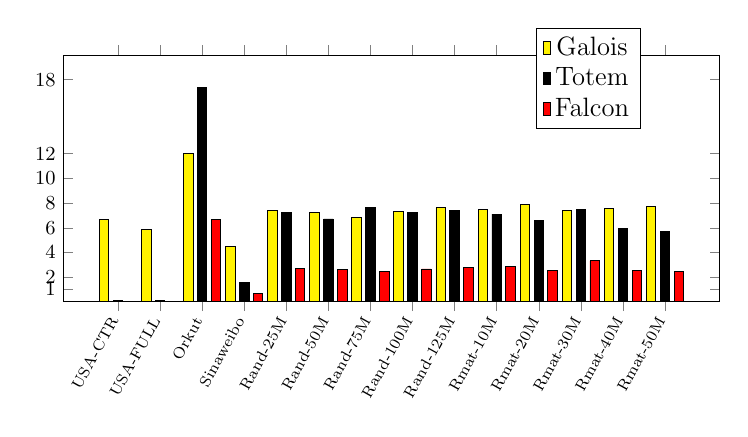
\begin{tikzpicture}[scale=0.8]
    \begin{axis}[
         ybar,% axis on top,
        ymin=0, ymax=20,
        height=5.5cm,
        width=12cm,
ytick={ 1,2,4,6,8,10,12,18},
%ymode=log,
 %       log basis y={2},
x tick label style={
rotate=60,anchor=east,font=\scriptsize},
        symbolic x coords={
           USA-CTR, USA-FULL, Orkut,Sinaweibo, Rand-25M,Rand-50M,Rand-75M,Rand-100M,Rand-125M, Rmat-10M,Rmat-20M,Rmat-30M,Rmat-40M,Rmat-50M
            },
       xtick=data,
        bar width=0.15cm,
%        major grid style={draw=black},
 %       enlarge y limits={value=.05,upper},
        % y tick style={grid=none},
         xticklabel style={rotate=1},
        %tickwidth=1pt,
       % enlarge x limits=true,
       legend style={
            at={(0.8,0.7)},
            anchor=south,
            legend columns=1,
           /tikz/every even column/.append style={font=\tiny}
        },
        legend entries={Lonestar-GPU,Falcon,Gunrock},
        legend image code/.code={%
      \draw[#1] (0cm,-0.1cm) rectangle (0.1cm,0.1cm);
   },  
        %ylabel={Speedup},
    %      nodes near coords,
  %nodes near coords align={vertical},
 every node near coord/.append style={color=black, rotate=90, anchor=south, font=\tiny},
             every axis/.append style={font=\small},
    ]
    \addplot [ fill=yellow] coordinates {
      (USA-CTR,6.67)
      (USA-FULL,5.86) 
      (Orkut, 12.01)
      (Sinaweibo,4.47)
      (Rand-25M,7.4)
      (Rand-50M,7.23) 
      (Rand-75M,6.82) 
      (Rand-100M,7.34) 
      (Rand-125M,7.62) 
      (Rmat-10M,7.5)
      (Rmat-20M,7.86) 
      (Rmat-30M,7.36) 
      (Rmat-40M,7.55) 
      (Rmat-50M,7.71) 
            };
    \addplot [ fill=black] coordinates {
      (USA-CTR,0.13)
      (USA-FULL,0.08) 
      (Orkut, 17.33)
      (Sinaweibo,1.55)
      (Rand-25M,7.25)
      (Rand-50M,6.71) 
      (Rand-75M,7.63) 
      (Rand-100M,7.26) 
      (Rand-125M,7.4) 
      (Rmat-10M,7.11)
      (Rmat-20M,6.59) 
      (Rmat-30M,7.49) 
      (Rmat-40M,5.96) 
      (Rmat-50M,5.69) 
            };
    \addplot [ fill=red] coordinates {
      (USA-CTR,0.02)
      (USA-FULL,0.02) 
      (Orkut, 6.68)
      (Sinaweibo,0.66)
      (Rand-25M,2.7)
      (Rand-50M,2.62) 
      (Rand-75M,2.44) 
      (Rand-100M,2.66) 
      (Rand-125M,2.78) 
      (Rmat-10M,2.87)
      (Rmat-20M,2.57) 
      (Rmat-30M,3.31) 
      (Rmat-40M,2.51) 
      (Rmat-50M,2.49) 
            };
 %\legend{Galois,Totem, Falcon}
 \legend{\large{Galois},\large{Totem}, \large{Falcon},\large{Green-Marl}}
 \end{axis}
   \end{tikzpicture}
\caption{CPU: Speedup over Galois single thread}
\label{expt:cccpucompare}
\end{subfigure}%
  \begin{subfigure}{0.4\textwidth}
   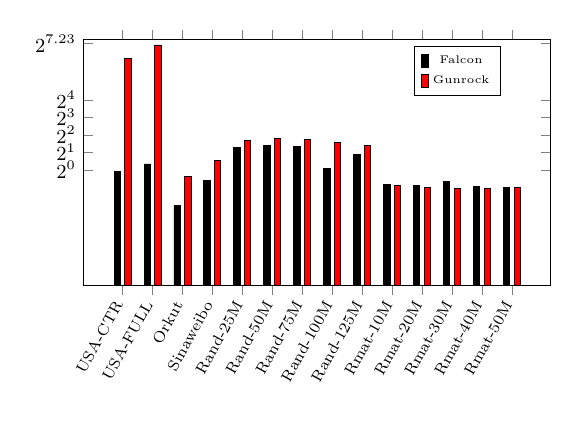
\begin{tikzpicture}[scale=0.8]
    \begin{axis}[
         ybar,% axis on top,
        ymin=0.01, ymax=180,
        height=5.5cm,
        width=9cm,
ymode=log,
log origin=infty,
        log basis y={2},
x tick label style={
rotate=60,anchor=east,font=\scriptsize},
        symbolic x coords={
           USA-CTR, USA-FULL, Orkut,Sinaweibo, Rand-25M,Rand-50M,Rand-75M,Rand-100M,Rand-125M, Rmat-10M,Rmat-20M,Rmat-30M,Rmat-40M,Rmat-50M
            },
       xtick=data,
ytick={0,1,2,4,8,16,150},
        bar width=0.1cm,
%        major grid style={draw=black},
 %       enlarge y limits={value=.05,upper},
        % y tick style={grid=none},
         xticklabel style={rotate=1},
        %tickwidth=1pt,
       % enlarge x limits=true,
       legend style={
            at={(0.8,0.77)},
            anchor=south,
            legend columns=1,
           /tikz/every even column/.append style={font=\tiny}
        },
        legend entries={Lonestar-GPU,Falcon,Gunrock},
        legend image code/.code={%
      \draw[#1] (0cm,-0.1cm) rectangle (0.1cm,0.1cm);
   },  
       % ylabel={Speedup},
    %      nodes near coords,
  %nodes near coords align={vertical},
 every node near coord/.append style={color=black, rotate=90, anchor=south, font=\tiny},
             every axis/.append style={font=\small},
    ]
    \addplot [ fill=black] coordinates {
      (USA-CTR,0.95)
      (USA-FULL,1.26) 
      (Orkut, 0.24)
      (Sinaweibo,0.65)
      (Rand-25M,2.40)
      (Rand-50M,2.65) 
      (Rand-75M,2.48) 
      (Rand-100M,1.07) 
      (Rand-125M,1.82) 
      (Rmat-10M,0.55)
      (Rmat-20M,0.53) 
      (Rmat-30M,0.64) 
      (Rmat-40M,0.52) 
      (Rmat-50M,0.49) 
            };
    \addplot [ fill=red] coordinates {
      (USA-CTR,84)
      (USA-FULL,142) 
      (Orkut, 0.78)
      (Sinaweibo,1.44)
      (Rand-25M,3.21)
      (Rand-50M,3.41) 
      (Rand-75M,3.33) 
      (Rand-100M,2.96) 
      (Rand-125M,2.63) 
      (Rmat-10M,0.53)
      (Rmat-20M,0.49) 
      (Rmat-30M,0.47) 
      (Rmat-40M,0.48) 
      (Rmat-50M,0.49) 
            };
 \legend{Falcon, Gunrock}
 \end{axis}
   \end{tikzpicture}
\caption{GPU: Speedup over Totem}
\label{expt:bfsgpucompare-log2}
\end{subfigure}
\caption{CC comparison}
\label{expt:cccpugpu}
  \end{figure*}


Figure~\ref{expt:ssspcpugpu}, Figure~\ref{expt:bfscpugpu} and Figrue~\ref{expt:cccpugpu} compares the performance of our modified Falcon against other frameworks.
For SSSP in GPU, we have observed that Falcon-generated code provides consistently better speedups compared to LonestarGPU and Gunrock, except on the two social networks (soc-orkut-dir and soc-sinaweibo).
Totem performs better on the social networks as well as on RMAT graphs due to its inbuilt edge-based processing and other optimizations to improve load-balancing across GPU threads.
In CPU version of SSSP, we have observed that Galois performs better than all other frameworks. Performance of Falcon, Totem and Green-Marl are similar.
For BFS in GPU, the results are mixed across various frameworks and there is no clear winner, but there are interesting patterns based on the graph types.
Gunrock performs quite well on the road networks (USA-road-USA and USA-road-CTR), primarily due to its work-efficient worklist-based processing.
Totem outperforms again on social networks due to edge-based processing and better load-balancing.
Performance of almost all the frameworks on RMAT graphs is quite similar, with LonestarGPU performing poorly.
Our Falcon stands out on random graphs with speedups close to 2$\times$ over all other frameworks.
In CPU, Totem is a clear winner for random and RMAT graphs whereas Galois performed better in road and social networks.
For GPU version of CC, Falcon performed better in road network, social network and random graphs. For RMAT graph, all the frameworks are similar.
In CPU version, performance of Galois and Totem are similar and better than Falcon.



\subsection{Effect of Vertex-based versus Edge-based}\label{expt:vertexedge}

\REM{
\begin{figure}
\centering
\includegraphics[width=0.99\linewidth]{GPU.pdf}
\includegraphics[width=0.99\linewidth]{CPU.pdf}
\caption{Edge-based versus vertex-based processing on GPU and CPU}
\label{speedup:gpu}
\label{speedup:cpu}
\end{figure}
}

\begin{figure*}
\centering
  \begin{subfigure}{0.45\textwidth}
  \centering
   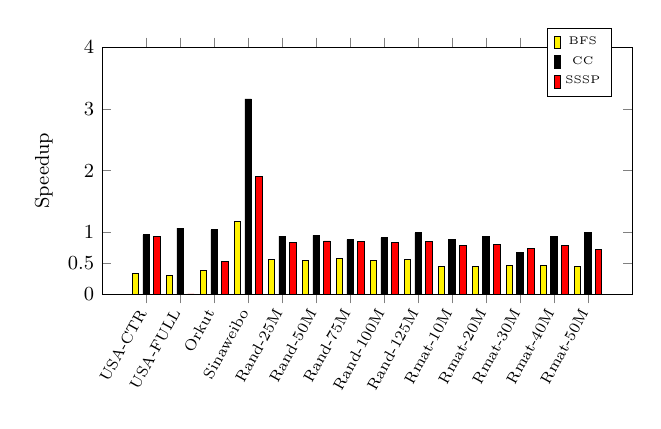
\begin{tikzpicture}[scale=0.8]
    \begin{axis}[
         ybar,% axis on top,
        ymin=0.001, ymax=4,
        height=5.5cm,
        width=10cm,
  ytick={ 0,0.5,1,2,3,4},
  x tick label style={
  rotate=60,anchor=east,font=\scriptsize},
        symbolic x coords={
           USA-CTR, USA-FULL, Orkut,Sinaweibo, Rand-25M,Rand-50M,Rand-75M,Rand-100M,Rand-125M, Rmat-10M,Rmat-20M,Rmat-30M,Rmat-40M,Rmat-50M
            },
       xtick=data,
        bar width=0.1cm,
%        major grid style={draw=black},
 %       enlarge y limits={value=.05,upper},
        % y tick style={grid=none},
         xticklabel style={rotate=1},
        %tickwidth=1pt,
       % enlarge x limits=true,
       legend style={
            at={(0.9,0.8)},
            anchor=south,
            legend columns=1,
           /tikz/every even column/.append style={font=\tiny}
        },
        legend entries={Lonestar-GPU,Falcon,Gunrock},
        legend image code/.code={%
      \draw[#1] (0cm,-0.1cm) rectangle (0.1cm,0.1cm);
   },  
        ylabel={Speedup},
    %      nodes near coords,
  %nodes near coords align={vertical},
 every node near coord/.append style={color=black, rotate=90, anchor=south, font=\normalsize},
             every axis/.append style={font=\small},
    ]
    \addplot [ fill=yellow] coordinates {
      (USA-CTR,0.33)
      (USA-FULL,0.30) 
      (Orkut, 0.38)
      (Sinaweibo,1.17)
      (Rand-25M,0.56)
      (Rand-50M,0.55) 
      (Rand-75M,0.57) 
      (Rand-100M,0.55) 
      (Rand-125M,0.56) 
      (Rmat-10M,0.45)
      (Rmat-20M,0.45) 
      (Rmat-30M,0.46) 
      (Rmat-40M,0.46) 
      (Rmat-50M,0.45) 
            };
    \addplot [ fill=black] coordinates {
      (USA-CTR,0.96)
      (USA-FULL,1.07) 
      (Orkut, 1.04)
      (Sinaweibo,3.16)
      (Rand-25M,0.94)
      (Rand-50M,0.95) 
      (Rand-75M,0.88) 
      (Rand-100M,0.91) 
      (Rand-125M,0.99) 
      (Rmat-10M,0.89)
      (Rmat-20M,0.93) 
      (Rmat-30M,0.67) 
      (Rmat-40M,0.94) 
      (Rmat-50M,0.99) 
            };
    \addplot [ fill=red] coordinates {
      (USA-CTR,0.93)
      (USA-FULL,0.0) 
      (Orkut, 0.53)
      (Sinaweibo,1.9)
      (Rand-25M,0.84)
      (Rand-50M,0.86) 
      (Rand-75M,0.85) 
      (Rand-100M,0.83) 
      (Rand-125M,0.85) 
      (Rmat-10M,0.78)
      (Rmat-20M,0.81) 
      (Rmat-30M,0.74) 
      (Rmat-40M,0.79) 
      (Rmat-50M,0.72) 
            };
 \legend{BFS,CC, SSSP}
 \end{axis}
   \end{tikzpicture}
\caption{CPU}
\label{expt:falconselfcpu}
\end{subfigure}\hfill
  \begin{subfigure}{0.45\textwidth}
      \centering
       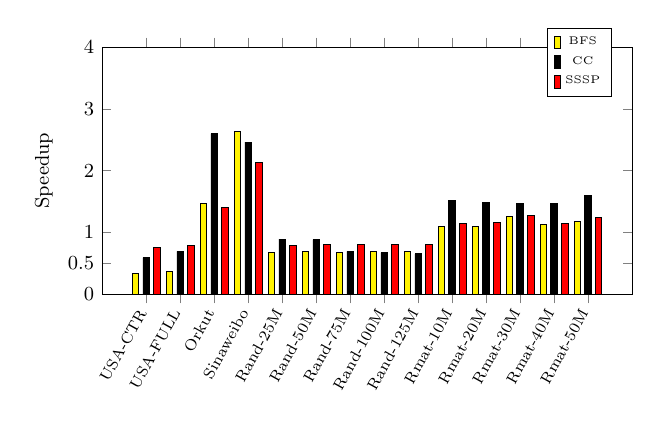
\begin{tikzpicture}[scale=0.8]
      \begin{axis}[
           ybar,% axis on top,
          ymin=0.001, ymax=4,
          height=5.5cm,
          width=10cm,
      ytick={ 0,0.5,1,2,3,4},
      x tick label style={
      rotate=60,anchor=east,font=\scriptsize},
            symbolic x coords={
               USA-CTR, USA-FULL, Orkut,Sinaweibo, Rand-25M,Rand-50M,Rand-75M,Rand-100M,Rand-125M, Rmat-10M,Rmat-20M,Rmat-30M,Rmat-40M,Rmat-50M
                },
           xtick=data,
            bar width=0.1cm,
    %        major grid style={draw=black},
     %       enlarge y limits={value=.05,upper},
            % y tick style={grid=none},
             xticklabel style={rotate=1},
            %tickwidth=1pt,
           % enlarge x limits=true,
           legend style={
                at={(0.9,0.8)},
                anchor=south,
                legend columns=1,
               /tikz/every even column/.append style={font=\tiny}
            },
            legend entries={Lonestar-GPU,Falcon,Gunrock},
            legend image code/.code={%
          \draw[#1] (0cm,-0.1cm) rectangle (0.1cm,0.1cm);
       },  
            ylabel={Speedup},
        %      nodes near coords,
      %nodes near coords align={vertical},
     every node near coord/.append style={color=black, rotate=90, anchor=south, font=\normalsize},
                 every axis/.append style={font=\small},
        ]
        \addplot [ fill=yellow] coordinates {
          (USA-CTR,0.34)
          (USA-FULL,0.37) 
          (Orkut, 1.47)
          (Sinaweibo,2.64)
          (Rand-25M,0.68)
          (Rand-50M,0.69) 
          (Rand-75M,0.68) 
          (Rand-100M,0.69) 
          (Rand-125M,0.69) 
          (Rmat-10M,1.1)
          (Rmat-20M,1.1) 
          (Rmat-30M,1.26) 
          (Rmat-40M,1.12) 
          (Rmat-50M,1.18) 
                };
        \addplot [ fill=black] coordinates {
          (USA-CTR,0.59)
          (USA-FULL,0.69) 
          (Orkut, 2.6)
          (Sinaweibo,2.46)
          (Rand-25M,0.89)
          (Rand-50M,0.88) 
          (Rand-75M,0.69) 
          (Rand-100M,0.67) 
          (Rand-125M,0.65) 
          (Rmat-10M,1.51)
          (Rmat-20M,1.48) 
          (Rmat-30M,1.47) 
          (Rmat-40M,1.46) 
          (Rmat-50M,1.60) 
                };
        \addplot [ fill=red] coordinates {
          (USA-CTR,0.75)
          (USA-FULL,0.78) 
          (Orkut, 1.41)
          (Sinaweibo,2.13)
          (Rand-25M,0.78)
          (Rand-50M,0.81) 
          (Rand-75M,0.81) 
          (Rand-100M,0.80) 
          (Rand-125M,0.80) 
          (Rmat-10M,1.14)
          (Rmat-20M,1.16) 
          (Rmat-30M,1.28) 
          (Rmat-40M,1.15) 
          (Rmat-50M,1.24) 
                };
     \legend{BFS,CC, SSSP}
     \end{axis}
       \end{tikzpicture}
    \caption{GPU}
    \label{expt:falconselfgpu}
  \end{subfigure}
\caption{Speedup of edge-based over vertex-based processing}
\label{expt:edgevertex}
\end{figure*}


Figure~\ref{expt:falconselfcpu} presents results of edge-based versus vertex-based processing of Falcon across various graphs for CC, BFS and SSSP. 
We observe that edge-based processing performs better in social-networks (soc-orkut-dir and soc-sinaweibo) and RMAT graphs. 
Both these kinds of graphs have skewed (power-law) degree-distribution resulting in large load-imbalance with vertex-based processing.
These graphs follow small-world property due to this peculiar (and natural) degree distribution.
On GPUs, this load-imbalance manifests itself as thread-divergence as the number of iterations (based on the number of neighbors) of each thread has high variance.
In other words, threads mapped to vertices having few neighbors have to wait for others mapped to high-degree vertices. 
This inhibits parallelism for SIMD style of processing.
In contrast, in edge-based processing, since threads are mapped to (a group of) edges, the load-imbalance is relatively negligible.
This results in better thread-divergence among warp-threads, leading to improved execution time.
Road networks and random graphs, on the other hand, have quite uniform degree-distribution.
Therefore, edge-based processing is not very helpful.
In fact, for uniform degree-distributions, edge-based processing may lead to inferior results (as seen in our experiments), due to increased synchronization requirement. %UK coaleased access will miss among threads in edge procesing on Graph in CSR??
Different outgoing edges of a vertex are processed sequentially by the same thread in vertex-based processing; whereas, those are processed in parallel by different threads.
Thus, edge-based processing necessitates more coordination among threads with respect to reading and updating attribute values of vertices.

Figure~\ref{expt:falconselfgpu} presents results of edge-based processing of Falcon on CPU.
We observe that, unlike on GPUs, edge-based processing is not helpful on GPUs. %UK-  GPUs->CPUs (last word in sentence
This is primarily due to CPUs not having enough resources to utilize the additional parallelism exposed by edge-based processing.
Thus, a few tens of threads perform in a similar manner in the presence of a million vertices or multi-million edges.
The only exception is soc-sinaweibo graph which witnesses over $3\times$ speedup for CC on CPU due to edge-based processing.
The improvements on this graph are also high for other algorithms as well (BFS and SSSP) compared to other graphs.
This occurs due to higher average degree in this social network (see Table~\ref{expt:chars}).%UK- orkut has more average degree ( |E| /|V|). Here |V| is low. variance in degree(1 to 33313) less   than orkut (1 to  278491).
Higher average degree adds sequentiality in vertex-based processing, while edge-based processing is not amenable to degree-distribution or average degree.
The overall effect gets pronounced for such dense graphs.

\subsection{Effect of Synchronous versus Asynchronous Processing}\label{expt:syncasync}
\begin{table}
\centering
\footnotesize
\begin{tabular}{|l|r|r|}
\hline
\textbf{Graph} & \textbf{Synchronous}  & \textbf{Asynchronous}\\
\hline
USA-road-CTR &	  86	& 91 	\\
USA-road-USA &	  134	& 106   \\
soc-orkut-dir &   425	& 285   \\
soc-sinaweibo &   8310	& 4508  \\
random-25M &   	  458	& 347   \\
random-50M &   	  945	& 741   \\
rmat-10M &   	  329	& 320   \\
rmat-20M &   	  771	& 665   \\
\hline
\textbf{Average}	&	1433	& 882	\\
\hline
\end{tabular}
\caption{Execution times (in ms) for Synchronous versus Asynchronous processing in CPU}
\label{tab:async-cpu}
\end{table}

Table~\ref{tab:async-cpu} presents the effect of asynchronous processing for various graphs on CPU.
We used a combination of BFS and SSSP to perform independent processing on the same graph.
We observe that asynchronous version improves execution time by 38\%. 
This occurs because threads do not have to wait for other threads.
This is primarily true on CPUs as threads are monolithically working on different parts of the graph and seldom require synchronization.
Such a processing is likely to benefit performance on GPUs as well, but due to limited GPU resources, the asynchronous kernels could not be executed together.
Therefore, our observed performance was the same for synchronous and asynchronous processing on GPUs (hence not shown again).

\subsection{Effect of Code Generation for Multiple Targets}\label{expt:cpugpu}

\begin{figure}
\begin{minipage}{0.45\textwidth}
\begin{table}[H]
\centering
\footnotesize
\begin{tabular}{|l|r|r|r|}
\hline
\textbf{Graphs} & \textbf{CPU-16} & \textbf{GPU} & \textbf{multi-GPU}\\\hline
random-25M + & 3866 & 1234 & 826 \\
random-50M		&	&	& \\\hline
rmat-10M + & 3024 & 1176 & 792 \\
rmat-20M	&	&	& \\
\hline
\end{tabular}
\caption{Execution time (in ms) of CC for two different graphs for various targets}
\label{tab:multigpu}
\end{table}
\end{minipage}\hfill
\begin{minipage}{0.45\textwidth}
\begin{table}[H]
\centering
\footnotesize
\begin{tabular}{|l|r|r|r|}
\hline
\textbf{Graphs} & \textbf{CPU-16} & \textbf{GPU} & \textbf{multi-GPU}\\\hline
USA-road-CTR + & 25363 & 12569 & 9138 \\
USA-road-USA	&	&	& \\\hline
soc-sinaweibo + & 4845 & 1503 & 1259 \\
soc-orkut-dir	&	&	& \\
\hline
\end{tabular}
\caption{Execution time (in ms) of BFS for two different graphs for various targets}
\label{tab:multigpumst}
\end{table}
\end{minipage}
\end{figure}

As discussed in Section~\ref{sec:cpugpu}, our approach can seamlessly generate code for CPU or GPU or multi-GPU.
The multi-GPU code works with different graphs for the same algorithm, or with the same graph for different algorithms.
Table~\ref{tab:multigpu} presents results for the former with CC as the algorithm generating code for CPU with 16 threads, single GPU and two GPUs, while Table~\ref{tab:multigpumst} presents those for BFS.
We observe that multi-GPU version took much less time as compared to other backends. 
In both CPU and single-GPU versions, the graphs are processed one after another.
On the other hand, in multi-GPU version, both the graphs are processed simultaneously in different GPUs; so the overall execution time is the larger of the two. 

\subsection{Effect of Data-Transfer Optimization}\label{expt:optimizations}
To illustrate the effect of the memcpy-optimization, we devised a simple Falcon program which computes BFS on GPU and then queries distances of various vertices from the CPU to compute the maximum distance.
We observe that the program with optimization takes less than a second to find the maximum distance.
On the other hand, without optimization the same program takes more than five minutes. 
This happens because without optimization, the existing Falcon engine generates code to copy distance of each vertex one by one as required in each iteration (total $N$ small \texttt{cudaMemcpy}s).
In contrast, the optimized code copies all the distances at once and then uses it for finding maximum distance (one large \texttt{cudaMemcpy}).
This leads to considerably reduced communication overhead, leading to improved execution.



%\subsection{Effect of Graph Type}\label{expt:graphtype}


\REM{
\begin{figure}
   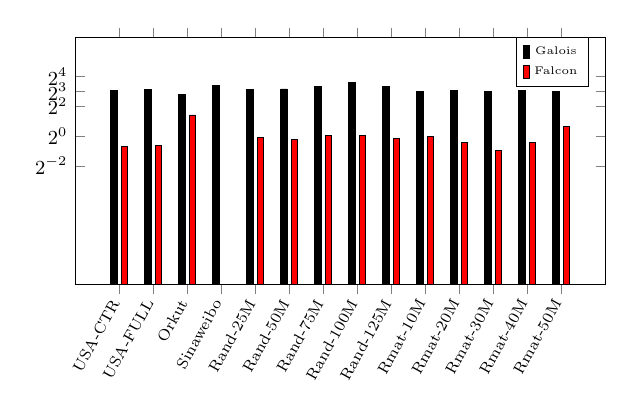
\begin{tikzpicture}[scale=0.8]
    \begin{axis}[
         ybar,% axis on top,
        ymin=0.001, ymax=100,
        height=5.5cm,
        width=10cm,
ytick={ 0.25,1,4,8,16},
ymode=log,
        log basis y={2},
log origin=infty,
x tick label style={
rotate=60,anchor=east,font=\scriptsize},
        symbolic x coords={
          % USA-CTR, USA-FULL, Orkut,Sinaweibo, Rand-25M,Rand-50M,Rand-75M,Rand-100M,Rand-125M, Rmat-10M,Rmat-20M,Rmat-30M,Rmat-40M,Rmat-50M
           USA-CTR, USA-FULL, Orkut,Sinaweibo, Rand-25M,Rand-50M,Rand-75M,Rand-100M,Rand-125M, Rmat-10M,Rmat-20M,Rmat-30M,Rmat-40M,Rmat-50M
            },
       xtick=data,
        bar width=0.1cm,
%        major grid style={draw=black},
 %       enlarge y limits={value=.05,upper},
        % y tick style={grid=none},
         xticklabel style={rotate=1},
        %tickwidth=1pt,
       % enlarge x limits=true,
       legend style={
            at={(0.9,0.8)},
            anchor=south,
            legend columns=1,
           /tikz/every even column/.append style={font=\tiny}
        },
        legend entries={Lonestar-GPU,Falcon,Gunrock},
        legend image code/.code={%
      \draw[#1] (0cm,-0.1cm) rectangle (0.1cm,0.1cm);
   },  
        %ylabel={Speedup},
    %      nodes near coords,
  %nodes near coords align={vertical},
 every node near coord/.append style={color=black, rotate=90, anchor=south, font=\normalsize},
             every axis/.append style={font=\small},
    ]
    \addplot [ fill=black] coordinates {
      (USA-CTR,8.44)
      (USA-FULL,8.88) 
      (Orkut, 7.09)
      (Sinaweibo,10.67)
      (Rand-25M,8.93)
      (Rand-50M,9) 
      (Rand-75M,10.24) 
      (Rand-100M,12.03) 
      (Rand-125M,10.11) 
      (Rmat-10M,7.94)
      (Rmat-20M,8.29) 
      (Rmat-30M,8.04) 
      (Rmat-40M,8.47) 
      (Rmat-50M,8.12) 
            };
    \addplot [ fill=red] coordinates {
      (USA-CTR,0.61)
      (USA-FULL,0.65) 
      (Orkut, 2.68)
      (Sinaweibo,0.001)
      (Rand-25M,0.92)
      (Rand-50M,0.86) 
      (Rand-75M,1.04) 
      (Rand-100M,1.03) 
      (Rand-125M,0.9) 
      (Rmat-10M,0.98)
      (Rmat-20M,0.75) 
      (Rmat-30M,0.52) 
      (Rmat-40M,0.74) 
      (Rmat-50M,1.60) 
            };
 \legend{Galois, Falcon}
 \end{axis}
   \end{tikzpicture}
\caption{MST speedup over Galois Single thread}
\label{expt:mstcpucompare}
\end{figure}
}



\REM{
  \begin{figure}
   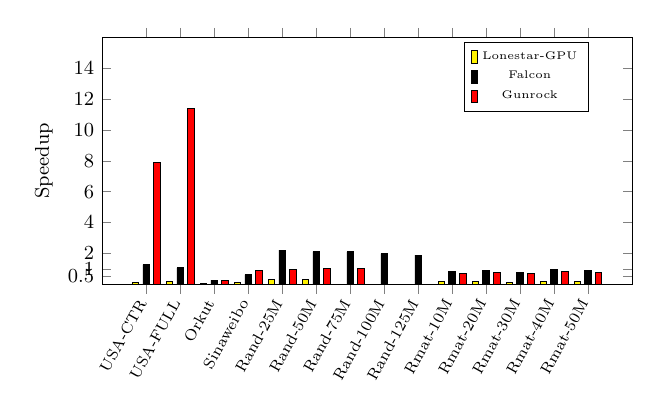
\begin{tikzpicture}[scale=0.8]
    \begin{axis}[
         ybar,% axis on top,
        ymin=0, ymax=16,
        height=5.5cm,
        width=10cm,
ytick={0.5, 1,2,4,6,8,10,12,14},
%ymode=log,
 %       log basis y={2},
x tick label style={
rotate=60,anchor=east,font=\scriptsize},
        symbolic x coords={
           USA-CTR, USA-FULL, Orkut,Sinaweibo, Rand-25M,Rand-50M,Rand-75M,Rand-100M,Rand-125M, Rmat-10M,Rmat-20M,Rmat-30M,Rmat-40M,Rmat-50M
  },
       xtick=data,
        bar width=0.1cm,
%        major grid style={draw=black},
 %       enlarge y limits={value=.05,upper},
        % y tick style={grid=none},
         xticklabel style={rotate=1},
        %tickwidth=1pt,
       % enlarge x limits=true,
       legend style={
            at={(0.8,0.7)},
            anchor=south,
            legend columns=1,
           /tikz/every even column/.append style={font=\tiny}
        },
        legend entries={Lonestar-GPU,Falcon,Gunrock},
        legend image code/.code={%
      \draw[#1] (0cm,-0.1cm) rectangle (0.1cm,0.1cm);
   },
        ylabel={Speedup},
    %      nodes near coords,
  %nodes near coords align={vertical},
 every node near coord/.append style={color=black, rotate=90, anchor=south, font=\tiny},
            every axis/.append style={font=\small},
    ]
    % \addplot [ pattern=crosshatch] coordinates {
    \addplot [ fill=yellow ] coordinates {
      (USA-CTR,0.14)
      (USA-FULL,0.19)
      (Orkut, 0.05)
      (Sinaweibo,0.13)
      (Rand-25M,0.3)
      (Rand-50M,0.28)
      (Rand-75M,0.001)
      (Rand-100M,0.001)
      (Rand-125M,0.001)
      (Rmat-10M,0.17)
      (Rmat-20M,0.15)
      (Rmat-30M,0.14)
      (Rmat-40M,0.19)
      (Rmat-50M,0.16)
            };
    \addplot [ fill=black] coordinates {
      (USA-CTR,1.26)
      (USA-FULL,1.059)
      (Orkut, 0.27)
     (Sinaweibo,0.62)
      (Rand-25M,2.2)
      (Rand-50M,2.11)
      (Rand-75M,2.09)
      (Rand-100M,1.98)
      (Rand-125M,1.89)
      (Rmat-10M,0.83)
      (Rmat-20M,0.9) 
      (Rmat-30M,0.76) 
      (Rmat-40M,0.95) 
      (Rmat-50M,0.86) 
            };
    % \addplot [ pattern=north east lines] coordinates {
    \addplot [ fill=red ] coordinates {
      (USA-CTR,7.89)
      (USA-FULL,11.39)
      (Orkut, 0.27)
      (Sinaweibo,0.88)
      (Rand-25M,0.98)
      (Rand-50M,1.01)
      (Rand-75M,1.02) 
      (Rand-100M,0.001)
     (Rand-125M,0.001)
      (Rmat-10M,0.71)
      (Rmat-20M,0.76)
      (Rmat-30M,0.70)
      (Rmat-40M,0.81) 
      (Rmat-50M,0.78) 
            };
 \legend{Lonestar-GPU,Falcon, Gunrock}
 \end{axis}
   \end{tikzpicture}
\caption{BFS speedup over Totem}
\label{expt:bfsgpucompare}
\end{figure} 
}


